\documentclass[a4paper,12pt]{article}
\usepackage{tabularx}
\usepackage{enumitem}
\usepackage{geometry}
\geometry{margin=1in}
\usepackage{booktabs} 
\usepackage{graphicx} % Required for inserting images
\usepackage{cite}
\bibliographystyle{IEEEtran}
 %Imports biblatex package
\usepackage{amsmath}     % For advanced math environments and symbols
\usepackage{amssymb}     % For additional math symbols (e.g., \mathbb)
\usepackage{graphicx}    % For including images (for the logo)
\usepackage{geometry}    % For easy page margin adjustment
\usepackage{makecell}    % For \makecell command in tables
\usepackage{url}         % For clean URLs in the document
\usepackage[table,xcdraw]{xcolor} % For colors in the table
\usepackage{changepage} % For centering the table on the whole page
\usepackage{float} % For putting the tables at the exact spot

\usepackage[colorinlistoftodos]{todonotes}
\usepackage{booktabs}
\usepackage{multirow}

% --- Pretty SDM helpers ---
\usepackage{colortbl}
\usepackage{array}
\usepackage{ragged2e}

% Compact bullets in tables
\newenvironment{tightitem}{%
  \begin{itemize}[leftmargin=*,label=--,topsep=1pt,itemsep=1.5pt,parsep=0pt]
}{\end{itemize}}

% Tiny provenance tags
\newcommand{\Ptag}{\textsf{\scriptsize[P]}} % prior solutions/competition
\newcommand{\Ttag}{\textsf{\scriptsize[T]}} % tech limit
\newcommand{\Dtag}{\textsf{\scriptsize[D]}} % design choice


\usepackage{fancyhdr}
\renewcommand\theadfont{\bfseries}
\renewcommand\cellalign{tl}
\setlist[itemize]{nosep,left=0pt,label=--,itemsep=2pt,topsep=2pt}
\renewcommand{\arraystretch}{1.35}
\setlength{\tabcolsep}{8pt}
\setlength{\arrayrulewidth}{0.6pt}
% Redefine the 'plain' style (used for page 1, chapter starts, etc.)
\makeatletter
\def\ps@plain{%
    \let\@mkboth\@gobbletwo
    \let\@oddhead\@empty
    \let\@evenhead\@empty
    \let\@evenfoot\@oddfoot
}
\makeatother

\pagestyle{plain} % Ensure all pages use this style

\newcommand{\coursename}{EE4C12 Machine Learning for Electrical Engineering Applications}
\newcommand{\projectname}{Project CE\_ARR }
\newcommand{\reporttype}{Final Report}
\newcommand{\groupmembers}{
\textbf Azat Idayatov,aidayatov@tudelft.nl (Student ID:6551505)\\
\textbf Giorgio Recchilongo, grecchilongo@tudelft.nl (Student ID: 6549632) \\
}

\begin{document}
\begin{titlepage}
\center

\vspace*{-12mm}

\includegraphics[width=62mm]{TUDelft_logo_rgb.png}
\vfill
\vfill

{\fontsize{60}{72}\selectfont\textbf{\projectname}}\\[6mm]{\Large \textbf{\reporttype}}\\

\vfill
\vfill

{\Large \textbf{\coursename}}\\[5mm]




{\large \groupmembers}
\vfill



\end{titlepage}

\section*{Summary}
This project aimed to classify different types of cardiac arrhythmias in patients through the analysis of ECG data and the creation of a machine learning model. \\Multiple model architecture were explored, including Multi-Layer-Perceprons (MLPs), Support Vector Machines (SVMs), Logistic Regression and tree-based ensembles (Random Forest, LightGBM). Techniques such as class weighting and SMOTE oversampling were used to address the class imbalance in the dataset.   \\
After hyperparameter tuning, the LightGBM model emerged as the best performer, achieving a macro-F1  score of 0.76 , a macro-accuracy of 0.98 and a macro-recall of 0.75 on the test set. These results demonstrate the effectiveness of gradient boosting for this specific unbalanced classification task. 


\section*{ML Pipeline}

\begin{figure}[h!]
\centering
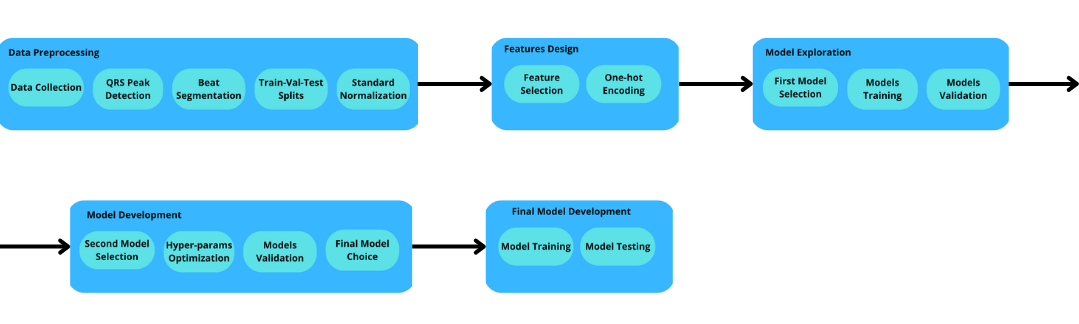
\includegraphics[width=1\textwidth]{Figs/pipeline.png}
\caption{Pipeline of the ML algorithm development}
\label{fig:pipeline}
\end{figure}
Figure \ref{fig:pipeline} shows the pipeline used in the development of the ML algorithm for this project.\\The first section is the Data Preprocessing: the data is acquired through ECG and the Pan Tompkins Algorithm is used for QRS peak detection. Subsequently, beat segmentation is performed on the signals in order to have a single instance of a beat per sample. Then the train, validation and test sets are created. These operations were performed prior to the start of the project.\\
The last step of the data-preprocessing section is data normalization: in our case a standard normalization, fitted on the training data in order to avoid data leakage, was applied to all the sample.\\\\
The next section is the Features Design, where one-hot encoding was performed on the target labels to avoid biasing the trained models.
\\\\
During the Model Exploration phase, various baseline models were trained and evaluated against the validation data. This operation provided an initial performance comparison, guiding our selection of the most beneficial models for further development.\\\\
Following the initial exploration, a subset of the best-performing models was selected for hyperparameter tuning. These optimized models were then re-evaluated on the validation set to determine the final model choice.
\\\\
For the final evaluation, the selected model was trained on the complete training dataset and then assessed against the unseen test set.

\section*{Task 1}
\subsection*{Model Selection}
\begin{itemize}[leftmargin=*]
    \item \textbf{Linear Models (Logistic Regression, LinearSVC)} These were selected to provide a computationally efficient and quick performance baseline and to test the hypothesis of linear separability in the data.

    \item \textbf{Non-Linear SVM (SVC with RBF kernel)} This was included to evaluate the effectiveness of a non-linear decision boundary, acknowledging that its computational complexity would likely be a limiting factor on the given dataset size.

    \item \textbf{Tree-Based Ensembles (RandomForest, LightGBM):} These models to explore whether a tree-based approach would be beneficial in our case, when they normally operate on more structured data. Random Forest, a bagging method, was used for its robustness, while LightGBM, a gradient boosting implementation, was selected for its efficiency on large datasets.

    \item \textbf{Multi-Layer Perceptron (MLP):} A deep learning approach was explored using the MLP. A baseline MLP was first established, followed by a systematic investigation of techniques to address the severe class imbalance, including sample weighting, SMOTE oversampling, and undersampling.
\end{itemize}

\subsection*{Performance Metrics}
In order to evaluate and compare the different types of models, performance metrics have to be taken into account. Considering the medical nature of the classification task, a higher priority was placed on minimizing the false negative rate over the false positive rate. This decision is justified by the clinical consequences: misclassifying a pathological sample as healthy poses a greater risk (the non-aknwoledgment of the disease) to the patient than a false positive, which would likely lead to further confirmatory testing. \\\\
At the same time, it was essential to avoid a strategy that simply flags all samples as pathological. While such an approach would achieve high recall, it is clinically impractical due to the overwhelming number of false positives it would generate. Consequently, the F1 score was selected as the primary evaluation metric because, as the harmonic mean of precision and recall, it provides a necessary balance between these two competing objectives. In cases where models achieved comparable F1 scores, recall was used as the deciding secondary metric.

\subsection*{Handling the Imbalanced Dataset}
A problem that was evident from the beginning was the train data set structure: although it presents an extremely high number of samples (more than 65,000), some target labels have a very low number of samples (as low as 2), as shown in Figure \ref{fig:train-dis}. This results in an extremely unbalanced dataset, where some strategies must be applied to get good results.\\In order to have reliable metrics that don't take into account the predominance of the "No disease" class, the metrics are always computed using the "macro" average, which treats every class as equally important, regardless of the number of samples.

\begin{figure}[h!]
\centering
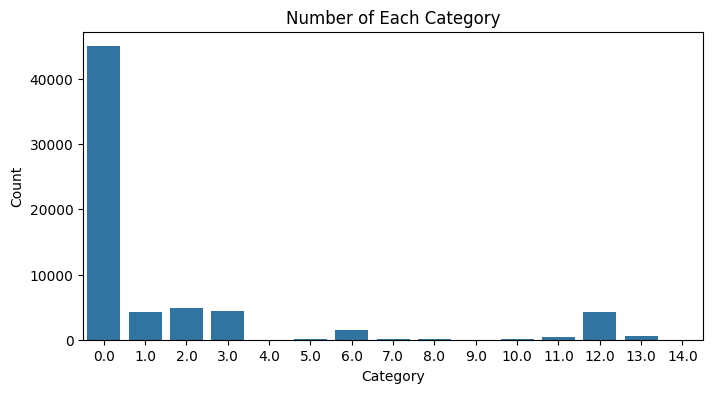
\includegraphics[width=0.8\textwidth]{Figs/train-set-distribution.png}
\caption{Sample class distribution}
\label{fig:train-dis}
\end{figure}

\subsection*{Results}
The model previously mentioned were trained on the training data and validated on the validation set. Table \ref{tab:model_comparison} shows the resulting performance metrics:
\begin{table}[htbp]
    \centering
    \caption{Comparison of baseline model performance metrics on the validation set. Recall and F1 scores are macro-averaged.}
    \label{tab:model_comparison}
    \begin{tabular}{lcc}
        \toprule
        \textbf{Model} & \textbf{Recall (Macro)} & \textbf{F1 (Macro)} \\
        \midrule
        Simple MLP & 0.37 & 0.38 \\
        Weighted MLP & 0.67 & 0.30 \\
        SMOTE MLP & 0.62 & 0.45 \\
        Downsampled MLP & 0.76 & 0.52 \\
        Forest search (Random Forest) & 0.73 & 0.57 \\
        Gradient boosting (LightGBM) & 0.68 & 0.72 \\
        SVC RBF & 0.86 & 0.61 \\
        Downsampled SVC RBF  & 0.79 & 0.49 \\
        SVC linear kernel & 0.59 & 0.30 \\
        Logistic regression & 0.69 & 0.35 \\
        \bottomrule
    \end{tabular}
\end{table}
\newpage
Overall, linear model, such as Linear SVC, and Logistic Regression performed poorly, indicating that the problem is not easily linearly-separable. On the other hand, the SVC model using the RBF kernel performed fairly good, although the high computational cost makes a further optimization too time-consuming.\\In addition, both tree-based approaches performed good, with the LightGMB model as the highest scoring for the F1 metric, combining this result with an extremely low computational time when compared to the others. \\
Finally, MLP had diverse results based on the strategies used to train them: while a simple MLP had bad overall scores, both weighting in a balanced way and synthetically oversampling through SMOTE improved dramatically the recall metric. \\Among the MLP models, a less orthodox strategy involving random undersampling of the "No disease" class to 10\% of its original size yielded the best performance. As shown in Table \ref{tab:model_comparison} under "Downsampled MLP", this approach achieved the highest recall and F1 scores within the MLP category.
\\\\

Figure \ref{fig:conf-simp-mlp} shows the confusion matrix of the simple MLP model and how it classifies most of the samples as "No disease" (class 0), thus scoring a low recall.\\
Figure \ref{fig:conf-rand-for} shows the confusion matrix of the Random Forest model, which has a better recall but, as clearly shown in the picture, the tendency of falsely flagging healthy samples as belonging to a pathological class.


\begin{figure}[h!]
\centering
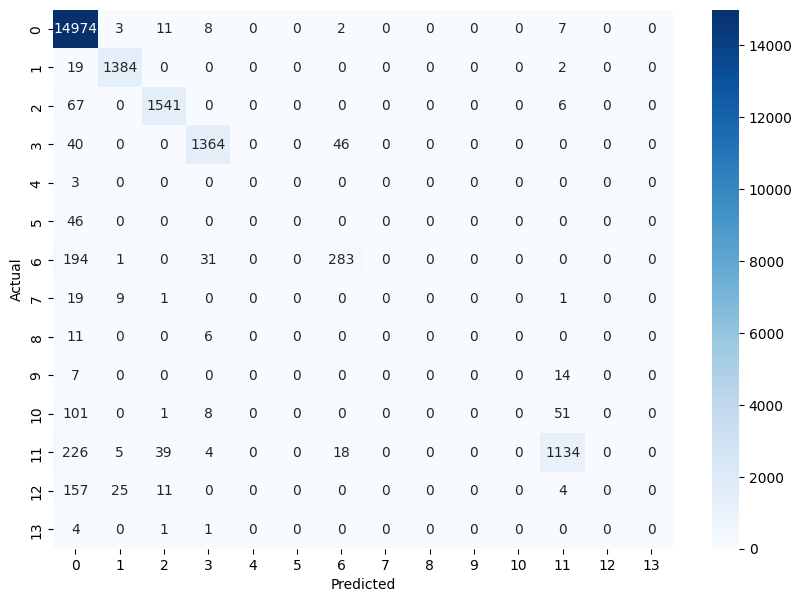
\includegraphics[width=0.8\textwidth]{Figs/conf-mat-simp-mlp.png}
\caption{Confusion matrix of the simple MLP model}
\label{fig:conf-simp-mlp}
\end{figure}
\newpage

\begin{figure}[h!]
\centering
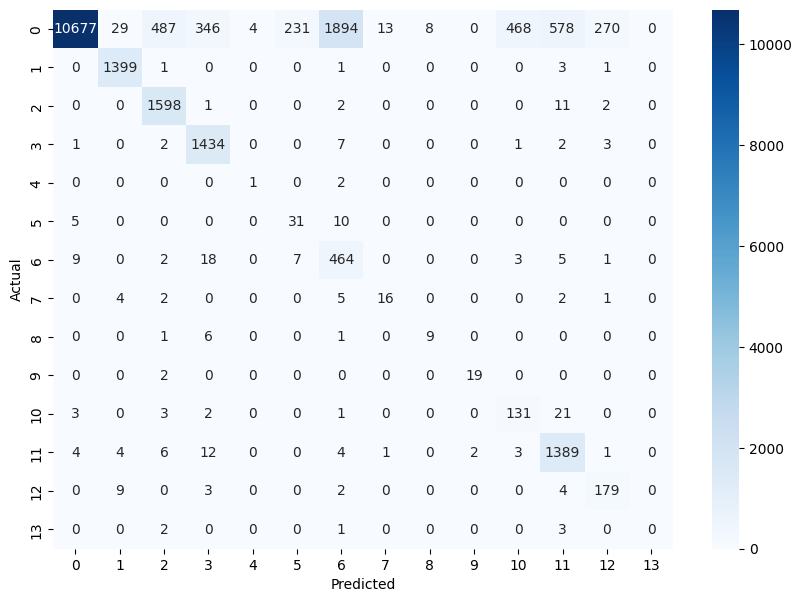
\includegraphics[width=0.8\textwidth]{Figs/conf-mat-rand-for.png}
\caption{Confusion matrix of Random Forest model}
\label{fig:conf-rand-for}
\end{figure}
\newpage




\section*{Task 2: Model Selection and Optimization}

In this task, we selected the most suitable models by comparing their accuracy, recall, and F1 scores, both before and after optimization. The models chosen for further analysis were:

\begin{enumerate}
    \item Downsampled MLP
    \item Random Forest
    \item Gradient Boosting (LightGBM)
\end{enumerate}

\subsubsection*{Performance Summary}

Table~\ref{tab:model_results} summarizes the macro and weighted recall and F1 scores \textbf{after optimization} for each model. For reference, Table~\ref{tab:model_preopt} presents the main metrics \textbf{before optimization}.

\begin{table}[h!]
    \centering
    \caption{Performance metrics before optimization}
    \label{tab:model_preopt}
    \begin{tabular}{lccc}
        \toprule
        \textbf{Model} & \textbf{Accuracy} & \textbf{Recall (Macro)} & \textbf{F1 (Macro)} \\
        \midrule
        Downsampled MLP & 0.90 & 0.80 & 0.55 \\
        Random Forest & 0.93 & 0.55 & 0.61 \\
        Gradient Boosting (LightGBM) & 0.94 & 0.69 & 0.68 \\
        \bottomrule
    \end{tabular}
\end{table}

\begin{table}[h!]
    \centering
    \caption{Performance metrics after optimization}
    \label{tab:model_results}
    \begin{tabular}{lccccc}
        \toprule
        \textbf{Model} & \textbf{Accuracy} & \textbf{Recall (Macro)} & \textbf{F1 (Macro)} & \textbf{Recall (W)} & \textbf{F1 (W)} \\
        \midrule
        Downsampled MLP & 0.88 & 0.76 & 0.50 & 0.85 & 0.88 \\ 
        Random Forest & 0.97 & 0.61 & 0.66 & 0.98 & 0.97 \\
        Gradient Boosting (LightGBM) & 0.98 & 0.71 & 0.72 & 0.98 & 0.98 \\
        \bottomrule
    \end{tabular}
\end{table}

\vspace{1em}

We now discuss each model's method and results in detail.

\paragraph{Downsampled MLP.}
\textbf{Method:} A Multilayer Perceptron (MLP) is a type of feedforward artificial neural network that consists of multiple layers of nodes. It is effective for capturing non-linear patterns in data. In this approach, we also downsampled the majority class(no disease, we left only 10\%) and used SMOTE to address class imbalance.

The MLP was configured with:
\begin{itemize}
    \item \texttt{hidden\_layer\_sizes} = (20, 10)
    \item \texttt{activation} = 'relu'
    \item \texttt{max\_iter} = 50
    \item \texttt{random\_state} = 42
\end{itemize}
Before optimization, this model achieved an accuracy of 0.90, macro recall of 0.80, and macro F1 score of 0.55. After optimization, the scores changed to accuracy = 0.88, macro recall = 0.76, and macro F1 = 0.50. Since the optimized results were lower, we decided to use the original configuration.

\begin{figure}[H]
    \centering
    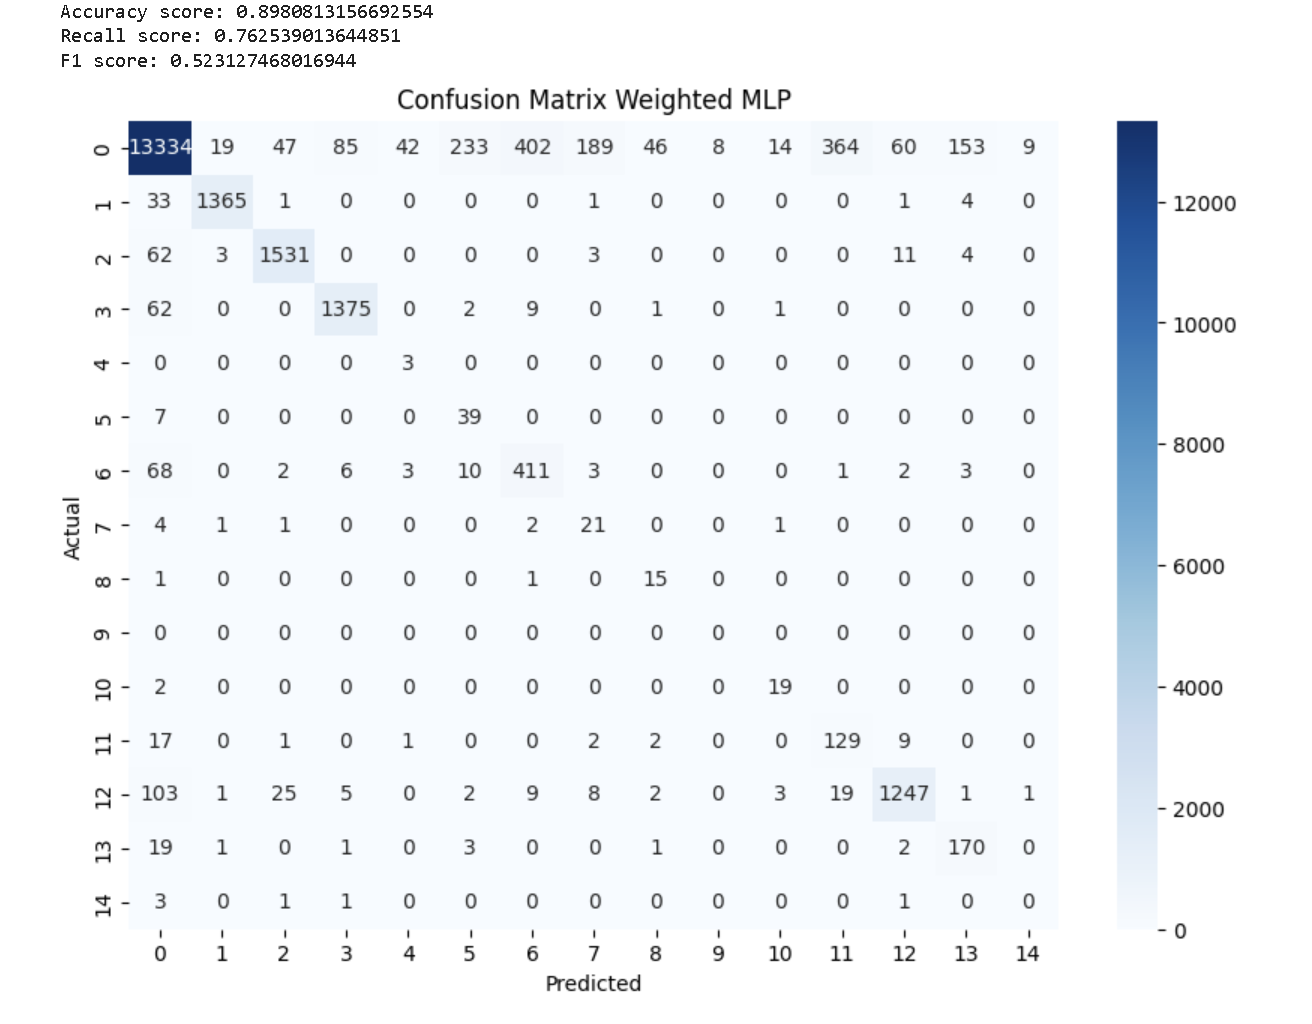
\includegraphics[width=0.8\textwidth]{Figs/conf_mat_downsamp.png}
    \caption{Confusion matrix of Downsampled MLP}
    \label{fig:conf_mat_downsamp}
\end{figure}

\paragraph{Random Forest.}
\textbf{Method:} Random Forest is an ensemble learning technique that constructs many decision trees during training and outputs the mode of the classes (classification) of the individual trees. It is robust to overfitting and effective for handling both categorical and numerical features.

The Random Forest model was trained using:
\begin{itemize}
    \item \texttt{class\_weight} = 'balanced'
    \item \texttt{n\_estimators} = 100
    \item \texttt{random\_state} = 42
\end{itemize}
Before optimization, the accuracy was 0.93, macro recall 0.55, and macro F1 score 0.61. After optimization, the model achieved accuracy = 0.97, macro recall = 0.61, and macro F1 = 0.66, with high weighted scores as well. This demonstrates strong overall performance, particularly on majority classes.

\begin{figure}[H]
    \centering
    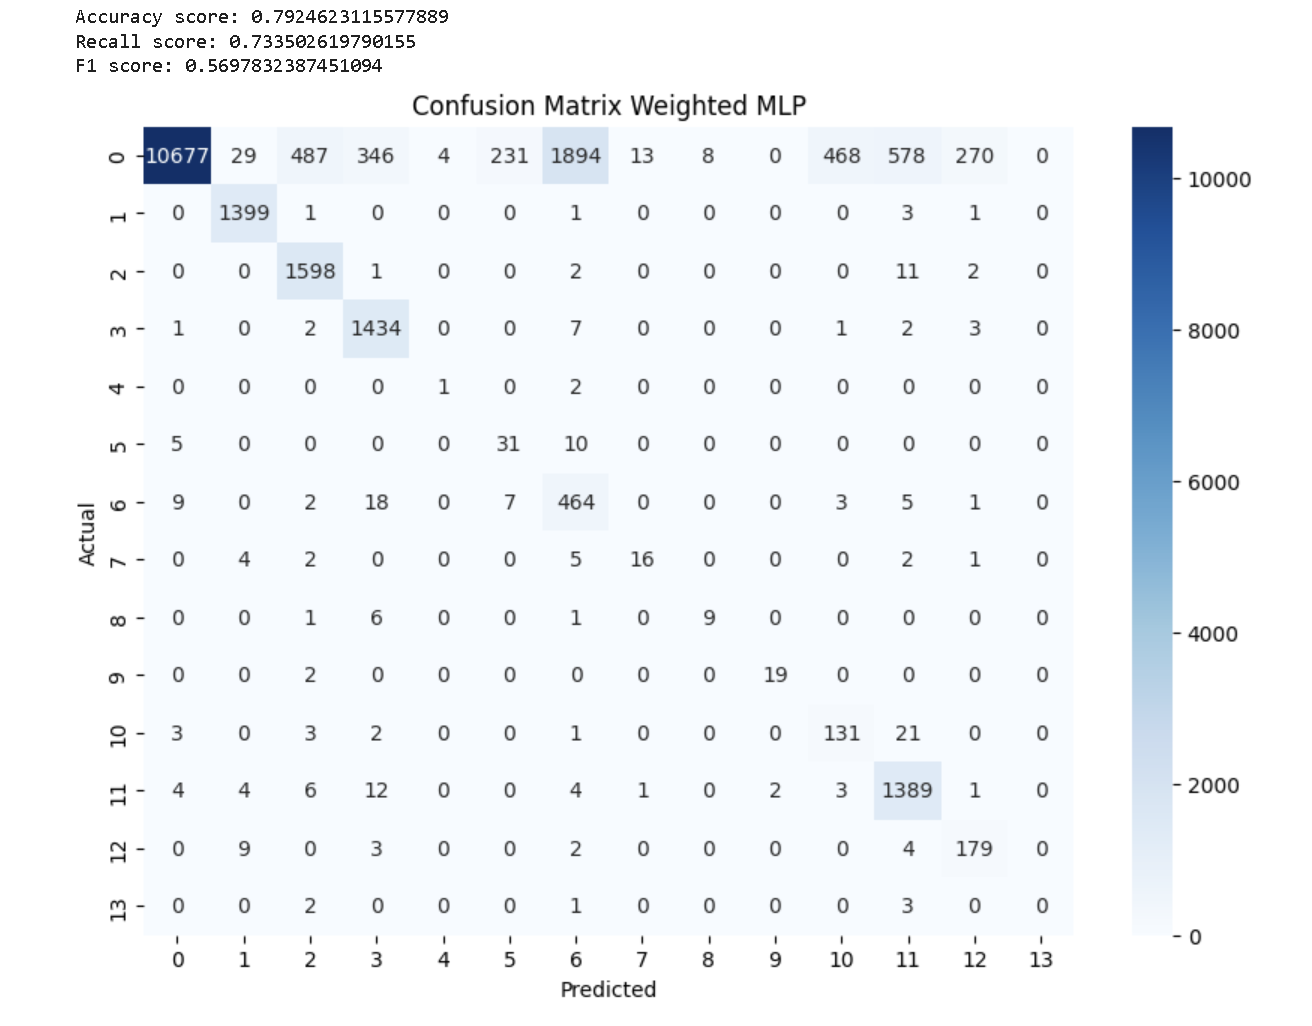
\includegraphics[width=0.8\textwidth]{Figs/Forest_search.png}
    \caption{Confusion matrix of Random Forest (after optimization)}
    \label{fig:conf_mat_rf}
\end{figure}

\paragraph{Gradient Boosting (LightGBM).}
\textbf{Method:} Gradient Boosting is an ensemble technique that builds models sequentially, where each new model tries to correct the errors of the previous one. LightGBM is an efficient implementation of gradient boosting that is particularly fast and effective for large datasets.

The LightGBM model was optimized with:
\begin{itemize}
    \item \texttt{class\_weight} = 'balanced'
    \item \texttt{n\_estimators} = 150
    \item \texttt{random\_state} = 42
    \item \texttt{n\_jobs} = 1
\end{itemize}
Pre-optimization metrics were accuracy = 0.94, macro recall = 0.69, macro F1 = 0.68. After optimization, the model achieved accuracy = 0.98, macro recall = 0.71, and macro F1 = 0.72, with weighted recall and F1 both at 0.98, indicating excellent performance across all classes.

\begin{figure}[H]
    \centering
    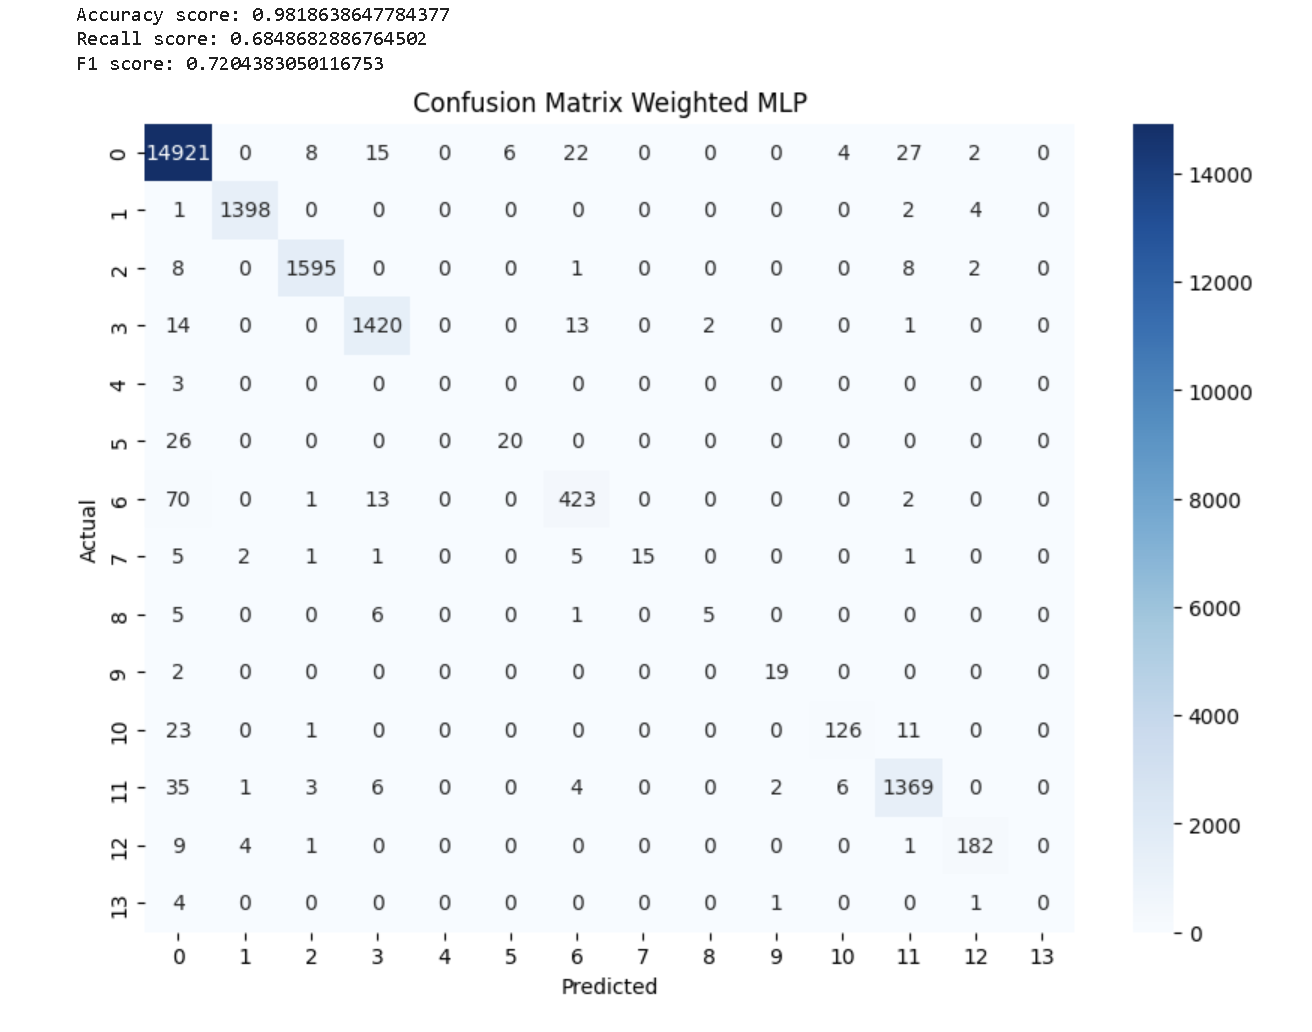
\includegraphics[width=0.8\textwidth]{Figs/Gradient_boosting.png}
    \caption{Confusion matrix of Gradient Boosting (LightGBM)}
    \label{fig:conf_mat_lgbm}
\end{figure}
\section*{Conclusion}

In this project, we systematically explored and compared a variety of machine learning models to address the challenging task of classifying arrhythmias from ECG data. The main challenge was the strong data imbalance, as no disease data prevailed on the disease data, this resulted in very high accuracy even with simple models, but with very low recall because the model can determine only no disease data, which make her useless.

Initial experiments with linear models like Logistic Regression and Linear SVC revealed their limitations, reflecting the underlying complexity and non-linearity of the classification problem. Non-linear approaches, particularly tree-based ensembles (Random Forest and LightGBM) and reduced sample neural networks (MLP), demonstrated considerably stronger performance. Among these, the LightGBM model emerged as the best overall performer after hyperparameter optimization, achieving a macro-F1 score of 0.72 and a macro-recall of 0.71 on the validation set, with exceptionally high weighted metrics as well.
To conclude, with the aid of different ML models and also with data modification, the problem of underselling of crucial data and class imbalance can be handled by overpopulating the rare class and applying more advanced model(as gradient boosting in our case).
\end{document}
